\documentclass[a4paper, 11pt]{article}
\usepackage{graphicx} % Required for inserting images

\usepackage[czech]{babel} %importování balíčku pro češtinu
\usepackage[T1]{fontenc} %specifikace fontu ze zadání
\usepackage[utf8]{inputenc}
\usepackage{times}
\usepackage{url}
\usepackage[hidelinks]{hyperref}
\usepackage{multicol}
\usepackage{multirow}
\usepackage{tabularray}

\usepackage[ruled, czech, linesnumbered, noline, longend]{algorithm2e}

\usepackage[left=20mm,text={170 mm, 240mm},top=30mm]{geometry} %nastavení okrajů stránky
\urlstyle{same}

\usepackage{pdflscape}
\usepackage{nolbreaks}



\begin{document}

\begin{titlepage}
    \begin{center}
            \Huge{\textsc{Vysoké učení technické v Brně}}\\ %[0.5em]
            \huge{\textsc{Fakulta informačních technologií}}\\
        
        \vspace{\stretch{0.382}}
        \LARGE{Typografie a publikování\,--\,3. projekt}\\
        \Huge{Tabulky a obrázky}
    \vspace{\stretch{0.618}}
    \end{center}
    {\Large{\today \hfill Hana Liškařová}}
\end{titlepage}

\section{Úvodní strana}
    Název práce umístěte do zlatého řezu a nezapomeňte uvést dnešní datum a vaše jméno a příjmení.

\section{Tabulky}
    Pro sázení tabulek můžeme použít buď prostředí\texttt{ tabbing }nebo prostředí\texttt{ tabular}. %Tu možná jinak mezery

    \subsection{Prostředí\texttt{ tabbing}}
        Při použití\texttt{ tabbing }vypadá tabulka následovně: %zase jinak mezery okolo tabbing
        \begin{tabbing}
            \qquad\qquad\qquad\quad  \=   \qquad\qquad  \= \kill
            \textbf{Ovoce}\> \textbf{Cena}  \> \textbf{Množství}\\
            Jablka        \> 25,90          \> 3 kg\\
            Hrušky        \> 27,40          \> 2,5 kg\\
            Vodní melouny  \> 35,--         \> 1 kus\\
        \end{tabbing}

        \noindent Toto prostředí se dá také použít pro sázení algoritmů, ovšem vhodnější je použít prostředí\texttt{ algorithm }nebo\texttt{ algorithm2e }(viz sekce \ref{Algoritmy}).

    \subsection{Prostředí\texttt{ tabular}}
    Další možností, jak vytvořit tabulku, je použít prostředí\texttt{ tabular}. Tabulky pak budou vypadat takto\footnote{Kdyby byl problém s\texttt{ cline}, zkuste se podívat třeba sem: \url{http://www.abclinuxu.cz/tex/poradna/show/325037}.}: \\

    
    \begin{table}[ht!]
        \catcode`\-=12
        \centering
        \begin{tabular}{| c | c | c |}
            \hline
               &  \multicolumn{2}{| c |}{\textbf{Cena}} \\ \cline{2-3} 
             \textbf{Měna} & \textbf{nákup} & \textbf{prodej}\\ \hline
             EUR & 25,475 & 27,045\\
             GPB & 28,835 & 30,705\\
             USD & 22,943 & 24,357\\ \hline
        \end{tabular}
        \caption{Tabulka kurzů k dnešnímu dni}
        \label{tab:Tabulka 1 }
    \end{table}

    \begin{table}[ht]
        \catcode`\-=12
        \centering
        \begin{tabular}{cccc}
            \begin{tabular}{|c|c|}
            \hline
               $A$  & $\neg{A}$ \\ \hline
                \textbf{P} & N \\ \hline
                \textbf{O} & O \\ \hline
                \textbf{X} & X \\ \hline
                \textbf{N} & P \\ \hline
            \end{tabular}
        &
            \begin{tabular}{|c|c|c|c|c|c|}
            \hline
               \multicolumn{2}{| c |}{\multirow{2}{*}{$A \land B$}}  &  \multicolumn{4}{| c |}{B}\\ \cline{3-6}
               \multicolumn{2}{| c |}{ }& \textbf{P} & \textbf{O} & \textbf{X} & \textbf{N} \\ \hline
               \multirow{4}{*}{$A$} & \textbf{P} & P & O & X & N \\ \cline{2-6}
               & \textbf{O} & O & O & N & N \\ \cline{2-6}
               & \textbf{X} & X & N & X & N \\ \cline{2-6}
               & \textbf{N} & N & N & N & N \\ \hline     
            \end{tabular}
        &
            \begin{tabular}{|c|c|c|c|c|c|}
            \hline
               \multicolumn{2}{| c |}{\multirow{2}{*}{$A \lor B$}}  &  \multicolumn{4}{| c |}{B}\\ \cline{3-6}
               \multicolumn{2}{| c |}{ }& \textbf{P} & \textbf{O} & \textbf{X} & \textbf{N} \\ \hline
               \multirow{4}{*}{$A$} & \textbf{P} & P & O & X & N \\ \cline{2-6}
               & \textbf{O} & P & O & P & O \\ \cline{2-6}
               & \textbf{X} & P & P & X & X \\ \cline{2-6}
               & \textbf{N} & P & P & P & P \\ \hline 
            \end{tabular}
        &
            \begin{tabular}{|c|c|c|c|c|c|}
            \hline
               \multicolumn{2}{| c |}{\multirow{2}{*}{$A \rightarrow B$}}  &  \multicolumn{4}{| c |}{B}\\ \cline{3-6}
               \multicolumn{2}{| c |}{ }& \textbf{P} & \textbf{O} & \textbf{X} & \textbf{N} \\ \hline
               \multirow{4}{*}{$A$} & \textbf{P} & P & P & P & P \\ \cline{2-6}
               & \textbf{O} & P & O & P & O \\ \cline{2-6}
               & \textbf{X} & P & P & X & X \\ \cline{2-6}
               & \textbf{N} & P & O & X & N \\ \hline
            \end{tabular}
        \\
        \end{tabular}
        
        \caption{ Protože Kleeneho trojhodnotová logika už je \uv{zastaralá}, uvádíme si zde příklad čtyřhodnotové logiky}
        \label{tab:Tabulka 2 }
    \end{table}
\pagebreak

\section{Algoritmy} \label{Algoritmy}
    Pokud budeme chtít vysázet algoritmus, můžeme použít prostředí\texttt{ algorithm\footnote{Pro nápovědu, jak zacházet s prostředím\texttt{ algorithm}, můžeme zkusit tuhle stránku: 
    \newline\url{http://ftp.cstug.cz/pub/tex/CTAN/macros/latex/contrib/algorithms/algorithms.pdf}.} }nebo\texttt{ algorithm2e\footnote{Pro\texttt{ algorithm2e }zase tuhle: \url{http://ftp.cstug.cz/pub/tex/CTAN/macros/latex/contrib/algorithm2e/doc/algorithm2e.pdf}.}}. Příklad použití prostředí\texttt{ algorithm2e }viz Algoritmus \ref{alg:Algoritmus 1}. \\

    \IncMargin{1.5em}
    \begin{algorithm} [ht]%DOPLNIT A OPRAVIT 
        \label{alg:Algoritmus 1}
        \caption{\textsc{FastSLAM}}
        
        \SetNlSty{}{}{:}
        \Indm
        \KwIn{$(X_{t-1}, u_t, z_t)$}
        \KwOut{$X_t$}
        \Indp
        \BlankLine
        $\overline{X_t}=X_t=0$\;
        \For{$k=1$ to $M$}{
        $x_t^{[k]} = sample\_motion\_model(u_t, x_{t-1}^{[k]})$\;
        $\omega_t^{[k]} = mesaurement\_model(z_t, x_{t}^{[k]}, m_{t-1})$\;
        $m_t^{[k]} = updated\_occupancy\_grid(z_t, x_{t}^{[k]}, m_{t-1}^{[k]})$\;
        $\overline{X_t}=\overline{X_t} + \langle x_{x}^{[m]}, w_{t}^{[m]} \rangle$\;
        }
        \For{$k=1$ to $M$}{
        draw $i$ with probability $\approx \omega_t^{[i]}$\;
        add $\langle x_{x}^{[k]}, m_{t}^{[k]}\rangle$ to $X_t$\;
        }
        \Return{$X_t$}  
        
    \end{algorithm}

\section{Obrázky}
    Do našich článků můžeme samozřejmě vkládat obrázky. Pokud je obrázkem fotografie, můžeme klidně použít bitmapový soubor. Pokud by to ale mělo být nějaké schéma nebo něco podobného, je dobrým zvykem takovýto obrázek vytvořit vektorově.
    
    \begin{figure}[!ht]
        \centering
        \scalebox{0.4}{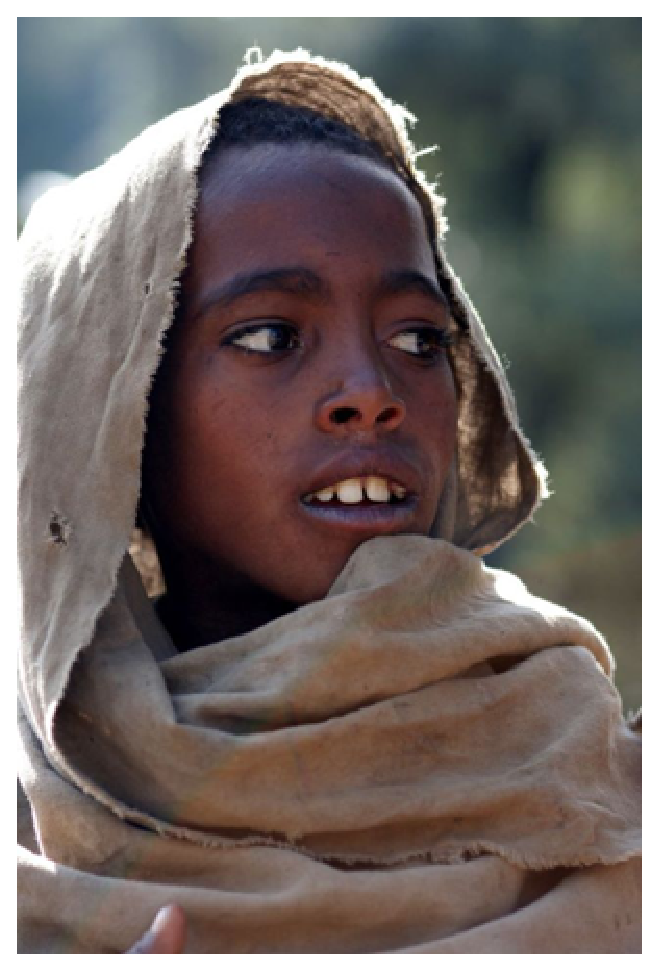
\includegraphics{etiopan.eps}
        \reflectbox{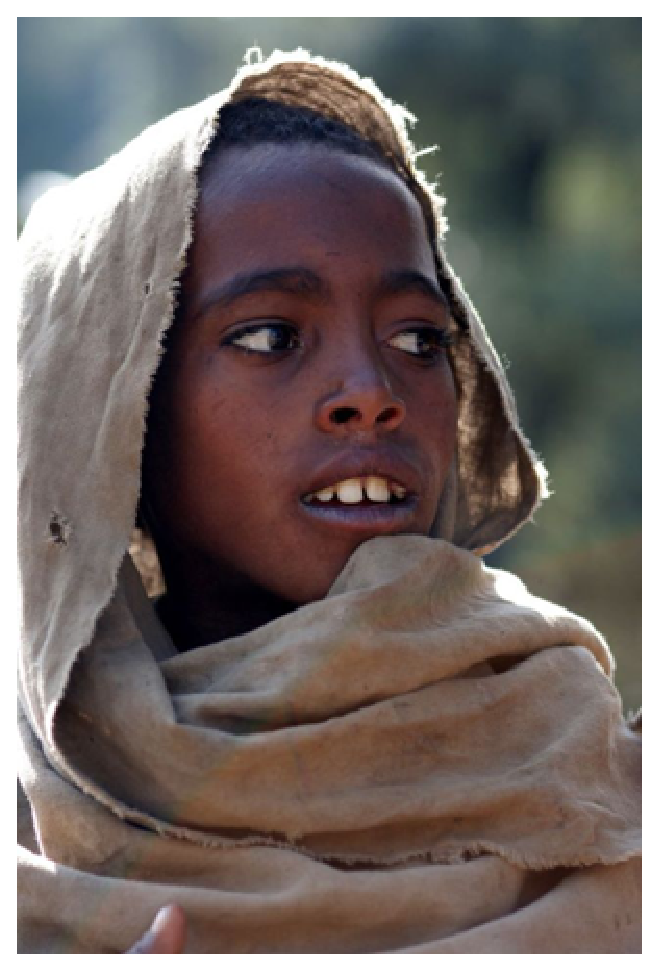
\includegraphics{etiopan.eps}} }
        \caption{Malý etiopiánek a jeho bratříček}
        \label{fig:Obrázek 1}
    \end{figure}
    
\pagebreak

    Rozdíl mezi vektorovým \dots

    \begin{figure}[!ht]
        \centering
        \scalebox{0.4}{
\includegraphics{oniisan.eps}}
        \caption{Vektorový obrázek}
        \label{fig:Obrázek 2}
    \end{figure}

    \noindent \dots a bitmapovým obrázkem
    
    \begin{figure}[!ht]
        \centering
        \scalebox{0.6}{
\includegraphics{oniisan2.eps}}
        \caption{Bitmapový obrázek}
        \label{fig:Obrázek 3}
    \end{figure}

    \noindent se projeví například při zvětšení.

    Odkazy (nejen ty) na obrázky \ref{fig:Obrázek 1}, \ref{fig:Obrázek 2} a \ref{fig:Obrázek 3}, na tabulky \ref{tab:Tabulka 1 } a \ref{tab:Tabulka 2 } a také na algoritmus \ref{alg:Algoritmus 1} jsou udělány pomocí křížových odkazů. Pak je ovšem potřeba zdrojový soubor přeložit dvakrát.

    Vektorové obrázky lze vytvořit i přímo v \LaTeX u, například pomocí prostředí\texttt{ picture}.



\begin{landscape}
    \begin{figure}
        \centering
        
    
    \begin{picture}(570, 280)
    \framebox(570,280)[0, 0]{ }
    
    \put(-80, 225){\circle{50}}
    \put(-440, 105){\framebox(390,20){ }}
    \put(-390, 125){\framebox(160,30){ }}
    \put(-230, 125){\framebox(145,5){ }}
    
    \put(-490,40){\line(0,1){100}}
    \put(-490,140){\line(1,0){100}}

    \put(-460,40){\line(0,1){35}}
    \put(-460,75){\line(1,0){90}}

    \put(-50,40){\line(0,1){20}}
    \put(-325,60){\line(1,0){275}}

    \put(-265,40){\line(-3,1){108}}

    \put(-410,75){\line(-1,1){30}}

    \put(-55,60){\line(0,1){40}}
    \put(-350,100){\line(1,0){295}}

    \put(-350,68){\line(0,1){32}}
    
    \linethickness{1mm}{\put(-550,40){\line(1,0){530}}}
    \end{picture}
    \caption{Vektorový obrázek moderního bydlení vhodného pro 21. století. (Buďto vytvořte stejný obrázek, anebo nakreslete pomocí picture váš vlastní domov.)}
    \label{fig:Obrázek 4}
    \end{figure}
\end{landscape}





\end{document}
